%! TeX root = rims-smooth-paper.tex
\documentclass[rims-smooth-paper.tex]{subfiles}
\begin{document}
\section{Implementation}
\label{sec:impl}

\begin{figure}[htbp]
  \centering
  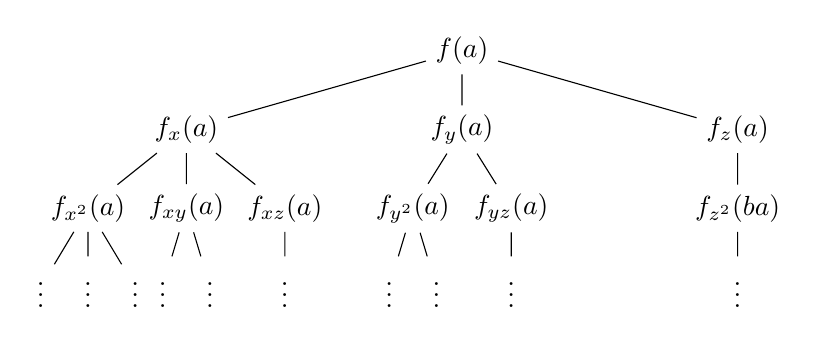
\begin{tikzpicture}[
    level/.style={level distance=1cm},
    level 1/.style={sibling distance=3.5cm},
    level 2/.style={sibling distance=1.25cm},
    level 3/.style={sibling distance=6mm}
    ]
    \newcommand{\ba}{\boldsymbol{a}}
    \node (fa) {$f(\ba)$}
      child{ 
        node (fxa) {$f_x(\ba)$}
          child { 
            node (fxxa) {$f_{x^2}(\ba)$}
            child {node{$\vdots$}}
            child {node{$\vdots$}}
            child {node{$\vdots$}}
          }
          child {
            node (fxya) {$f_{xy}(\ba)$}
            child {node{$\vdots$}} child {node{$\vdots$}}
          }
          child { 
            node (fxza) {$f_{xz}(\ba)$}
            child { node{$\vdots$} }
          }
      }
      child {
        node (fya) {$f_y(\ba)$}
        child { node {$f_{y^2}(\ba)$} child {node{$\vdots$}} child{ node{$\vdots$}} }
        child { node {$f_{yz}(\ba)$} child {node {$\vdots$}} }
      }
      child {
        node (fza) {$f_z(\ba)$}
        child {
            node {$f_{z^2}(ba)$}
            child { node {$\vdots$} }
        }
      };
  \end{tikzpicture}
  \caption{Ternary case\label{fig:tree}}
\end{figure}

\begin{listing}[tbp]
\begin{code}
data STower n a where
  ZS :: !a -> STower 0 a
  SS :: !a -> STower (n + 1) a -> STower n a -> STower (n + 1) a

liftSTower
  :: forall c n a. (KnownNat n, c a, forall x k. c x => c (STower k x) )
  => (forall x. c x => x -> x)
      -- ^ Function
  -> (forall x. c x => x -> x)
      -- ^ its first-order derivative
  -> STower n a
  -> STower n a
liftSTower f df (ZS a) = ZS (f a)
liftSTower f df x@(SS a da dus)
  = SS (f a) (da * df x) 
       (liftSTower @c f df dus)
\end{code}
\caption{Core definitions\label{lst:data-def}}
\end{listing}

\end{document}